\setsection{Méthode des Points Distincts et ses variantes}
	Comme nous l'avons vue précédement la méthode des points distincts introduites en 1982 \cite{Rivest}, consiste à fixer un critère d'arrêt. Ainsi, nous vérifions si le dernier élément de la chaîne se trouve dans une table seulement s'il respecte le même critère d'arrêt, limitant de ce fait le nombre de ces vérification.

	\bigskip

	Cette technique semble avoir un intérêt limité pour les \glspl{rainbow}. Mais de nombreuses recherches ont été mené menant a des solutions novatrice.

	\bigskip

	\setsubsection{Méthodes des points distincts}

		Comme nous l'avons vue, nous créons des chaînes de taille variable, mais nous fixons des bornes par sécurité. En effet une chaîne peut réaliser une boucle en fusionnant avec elle-même et par conséquant ne jamais vérifier la condition d'arrêt. C'est pourquoi nous posons $\hat{t}=t_{max}$ la limite haute avant d'écarter une chaîne. De même, nous fixons une limite basse $\check{t}=t_{min}$ afin d'éviter d'avoir des chaînes trop courte. Ainsi nous pouvons appliqué la méthode des points distincts aux \glspl{rainbow} en fixant $\hat{t}$ fonctions de réduction. Toutes ne seront pas utilisés, mais nous en auront le minimun requis pour appliquer cette technique.

		\bigskip

		Etant donné que les chaînes des tables s'arrêtent au premier point distinct compris dans les bornes, si nous ne trouvons pas de correspondance entre la chaîne que nous générons et une table, alors nous pouvons être sûr que notre clé ne se trouve pas dans cette table. Ainsi par table, nous ne réalisons qu'une seule vérification. Le nombre de vérification nécessaire est estimé être réduit par un facteur de $2^d$ où $d=\frac{1}{3}\log_2 N$

		\bigskip

		Le plus gros défaut de cette technique est la nécessité de stocker la taille des chaînes, ce qui rajoute un coût non-négligeable. C'est une des raisons pour lesquelles cette technique n'apporte que peu d'avantage en essayant de l'appliquer aux \glspl{rainbow}.

		\bigskip

	\setsubsection{Première Variante}

		Une première idée proposé dans cet article \cite{VDP}, est de faire varier la condition d'arrêt en fonction du point de départ. L'un des avantages est qu'ainsi nous avons des informations sur le point de départ dans le point final. La conséquence est que nous ne sommes plus obliger de stocker le point de départ.

		\bigskip

		Malheureusement cette technique ne semble pas plus efficace qu'une \gls{rainbow} classique \cite{VDP,Wang}. Nous avons d'ailleurs les résultats d'une analyse théorique dans le tableau proposé par \cite{VDP} joint ci-dessous.

		\bigskip

		\newcommand{\extheight}{\rule[-9pt]{0pt}{25pt}}

		\begin{owntab}{l*{4}{|L{25mm}}}
			& nombre d'entrée par table ($M$)	& nombre de recherche dans la table	& nombre d'évaluations de fonction	& équation de la courbe de compromis	\\\hline
			Hellman			& $mt$ & $t^2$					& $t^2$					 & $TM^2=N^2$				\extheight{}\\\hline
			Arc-en-ciel		& $mt$ & $t$					& $\frac{1}{2}t^2$		 & $TM^2=\frac{1}{2}N^2$	\extheight{}\\\hline
			Hellman+DP		& $mt$ & $t$					& $\frac{1}{2}t^2$		 & $TM^2=\frac{1}{2}N^2$	\extheight{}\\\hline
			Hellman+VDP		& $mt$ & $t*\hat{t}$			& $t*\hat{t}$			 & $TM^2=c*N^2$				\extheight{}\\\hline
			Arc-en-ciel+DP	& $mt$ & $\hat{t}$				& $\frac{1}{2}\hat{t}^2$ & $TM^2=\frac{c^2}{2}N^2$	\extheight{}\\\hline
			Arc-en-ciel+VDP	& $mt$ & $\frac{1}{2}\hat{t}^2$	& $\frac{1}{2}\hat{t}^2$ & $TM^2=\frac{c^2}{2}N^2$	\extheight{}\\
		\end{owntab}

		\bigskip

		Où nous avons $\hat{t}=t_{max}=c*t$, de plus ces donnés sont calculés selon le pire des cas. Mais comme nous pouvons le constater le facteur c a de forte chance de limiter l'intérêt de ces tables. Ainsi dans l'article \cite{VDP}, les auteurs ont cherché les paramètres optimaux pour rendre cette technique viable, mais ils n'y sont pas parvenue.

	\setsubsection{Les tables arc-en-ciel floues}

		Une autre alternative a été proposé \cite{fuzzy} dont l'idée consiste à agréger différntes de tables de Hellman associé à la technique des points distincts. Nous obtenons ainsi une \gls{rainbow} où en lieu et place de changer de fonction de réduction pour chaque colonne, nous en changeons à chaque fois que nous respectons le critère d'arrêt. Nous obtenons alors le modèle ci-dessous. La mise en place plus pratique a été étudié par \cite{fuzzyStudy}
\begin{figure}[h!]
	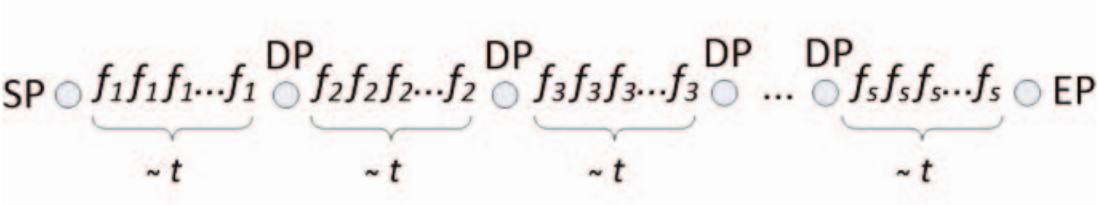
\includegraphics[width=0.9\linewidth]{other/fuzzy.png}
\end{figure}

	\setsubsection{Conclusion}

		La méthode des points distincts est encore aujourd'hui exploré mais jusqu'à présent elle n'a pas donné de résultat probant. Une autre méthode pour limiter le coût des recherches dans les tables a été présenté par \cite{checkpoints} en 2005. C'est une méthode basé sur des points de contrôle. Nous la verrons plus en détail dans la prochaine section
		
\endinput{}
